%IMPORTS
\documentclass[a4paper, 11pt]{article}
\usepackage[utf8]{inputenc} 
\usepackage[T1]{fontenc}
\usepackage[catalan]{babel}
\usepackage{amsmath, amssymb, amsthm}
\usepackage[margin=1in]{geometry}
\usepackage{enumerate}
\usepackage{array}
\usepackage{graphicx}
\usepackage{wrapfig}
\usepackage{ragged2e} 
\usepackage{subfig}
\usepackage{caption}
\usepackage{subcaption}
\usepackage[dvipsnames]{xcolor}
%\usepackage[table]{xcolor}
\usepackage{float}
\usepackage{chngcntr}
\usepackage{ragged2e}
\usepackage{multirow}
\usepackage{vmargin}
\usepackage{hyperref}
\usepackage{url}
\usepackage{fancyhdr}
\usepackage{bigints}
\usepackage{listings}
\usepackage{xcolor,colortbl}
\usepackage{enumitem}
% \usepackage[english, spanish]{babel}
% \usepackage{slashbox}
\usepackage{diagbox}


\definecolor{navy}{rgb}{0,0,128}
\definecolor{codegreen}{rgb}{0,0.6,0}
\definecolor{codegray}{rgb}{0.5,0.5,0.5}
\definecolor{codepurple}{rgb}{0.58,0,0.82}
\definecolor{backcolour}{rgb}{0.95,0.95,0.92}
\definecolor{amaranth}{rgb}{0.9, 0.17, 0.31}
\definecolor{GRAY}{rgb}{0.75, 0.75, 0.75}


\lstdefinelanguage{Sage}[]{Python}
{morekeywords={False,sage,True},sensitive=true}
\lstset{
  frame=none,
  showtabs=False,
  showspaces=False,
  showstringspaces=False,
  commentstyle={\ttfamily\color{dgreencolor}},
  keywordstyle={\ttfamily\color{dbluecolor}\bfseries},
  stringstyle={\ttfamily\color{dgraycolor}\bfseries},
  language=Sage,
  basicstyle={\fontsize{10pt}{10pt}\ttfamily},
  aboveskip=0.3em,
  belowskip=0.1em,
  %numbers=left,
  numberstyle=\footnotesize
}
\definecolor{dblackcolor}{rgb}{0.0,0.0,0.0}
\definecolor{dbluecolor}{rgb}{0.01,0.02,0.7}
\definecolor{dgreencolor}{rgb}{0.2,0.4,0.0}
\definecolor{dgraycolor}{rgb}{0.30,0.3,0.30}
\newcommand{\dblue}{\color{dbluecolor}\bf}
\newcommand{\dred}{\color{dredcolor}\bf}
\newcommand{\dblack}{\color{dblackcolor}\bf}

\lstset{
morekeywords={var}
}
\lstset{
morekeywords={imag}
}
\lstset{
morekeywords={real}
}
\lstset{
morekeywords={contour\_plot}
}
\lstset{
morekeywords={streamline\_plot}
}
\lstset{
morekeywords={show}
}
\lstset{
morekeywords={plot\_vector\_field}
}

\setpapersize{A4}
\setmargins{2.5cm}     % margen izquierdo
{2.6cm}                % margen superior
{16.5cm}               % anchura del texto
{23.7cm}               % altura del texto
{10pt}                 % altura de los encabezados
{0cm}                  % espacio entre el texto y los encabezados
{0pt}                  % altura del pie de página
{1cm}                  % espacio entre el texto y el pie de página
\renewcommand{\baselinestretch}{1.5}

\begin{document}

\begin{titlepage}
    \centering
    {\bfseries\LARGE Universitat Autònoma de Barcelona\newline Facultat de Ciències\par}
    \vspace{2cm}
    {\hspace{-1em}
\includegraphics[width=0.4\textwidth]{logo.png}\par}
    \vspace{1cm}
    {\scshape\Huge Seminari 2: Fluids\par} 
    \vspace{1cm}
    {\Large \itshape Autors: \par}
    {\Large  Gerard Lahuerta \& Ona Sánchez \& Andrea González \par}
    {\Large 1601350 --- 1601181 --- 1603921 \par}
    \vspace{1cm}
    {\Large 29 d'Abril del 2022\par}
\end{titlepage}

\justifying

\newpage
\setcounter{page}{2}
\pagestyle{plain}
\tableofcontents
\cleardoublepage
\addcontentsline{}{chapter}{}
\newpage


\section{Exercici 2.4.13}
Modifiquem el flux amb potencial donat per $f(z) = \log(z+2)$ que és una font sortint des del punt $(z = -2)$ (vist en un exemple/exercici anterior). Per això considerem la modificació donada pel potencial:
    \begin{equation*}
    \Phi(z) = f(z) + \overline{f\left(\frac{1}{\overline{z}}\right)} = \log(z+2) + \overline{\log\left(\frac{1}{\overline{z}}+2\right)}
\end{equation*}
     \begin{enumerate}[label=(\alph*)]
         \item \textbf{Descomposar $\Phi(z)$ en fluxos coneguts.}
         \begin{equation*}
            \begin{split}
                 \Phi(z) & = f(z) + \overline{f\left(\frac{1}{\overline{z}}\right)}\\
                        & = \log(z+2) + \overline{\log\left(\frac{1}{\overline{z}}+2\right)}\\
                        & = \log(z+2) + \log\left(\frac{1}{z}+2\right)\\
                        & = \log(z+2) + \log\left(\frac{1+2z}{z}\right)\\
                        & = \log(z+2) + \log(1+2z) - \log(z)\\
                        & = \log(z+2) + \log\left( 2\cdot \left(\frac{1}{2}+z\right)\right) - \log(z)\\
                        & = \log(z+2) + \log\left(\frac{1}{2}+z\right) - \log(z) + \log(2)
            \end{split}
        \end{equation*}
         \item \textbf{Calcular $\Phi '(z)$ i confirmar el que es demostra a l'apartat anterior.}
     
        \begin{itemize}
            \par
            \item Càlcul de la derivada de $\Phi$:
            \begin{equation*}
            \begin{split}
                 \Phi'(z) & = \left(f(z) + \overline{f\left(\frac{1}{\overline{z}}\right)}\right)'\\
                 & = \left(\log(z+2) + \log\left(\frac{1}{2}+z\right) - \log(z) + \log(2)\right)'\\
                 & = \frac{1}{z+2} + \frac{1}{\frac{1}{2}+z} - \frac{1}{z}
            \end{split}
        \end{equation*}
            \item Comprovació de l'apartat anterior:\\
            Usant l'expressió obtingut a l'apartat \textit{(a)}: $\log(z+2) + \log\left(\frac{1}{2}+z\right) - \log(z) + \log(2)$, trobem $3$ punts singulars situats a: $z=-2$, $z=-\frac{1}{2}$ i $z=0$.\\
            Sabem que per $\Phi(z) = k\cdot\log(z-a)$, quan $k > 0$ es forma una $font$, i quan $k < 0$ una $pica$.
            \newpage
            Estudiem els diversos punts singulars:
            \begin{enumerate}
                \item $z=-\frac{1}{2}$: S'obté de $\log\left(\frac{1}{2}+z\right)$. En aquest cas, $k=1 \rightarrow k>0$, per tant en el $-\frac{1}{2}$ es troba una $font$.
                \item $z=0$: S'obté de $- \log(z)$. En aquest cas, $k=-1 \rightarrow k<0$, per tant en el $0$ es troba una $pica$.
                \item $z=-2$: S'obté de $\log(z+2)$. En aquest cas, $k=1 \rightarrow k>0$, per tant en el $-2$ es troba una $font$.

            \end{enumerate}
            
            
            \begin{figure}[h]
                 \centering
                  \subfloat{
                   \label{f:gato}
                    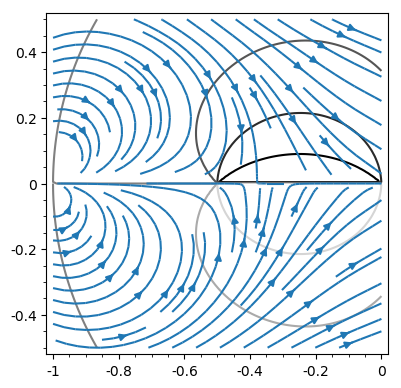
\includegraphics[width=0.3\textwidth]{B-0.png}}
                  \subfloat{
                   \label{f:tigre}
                    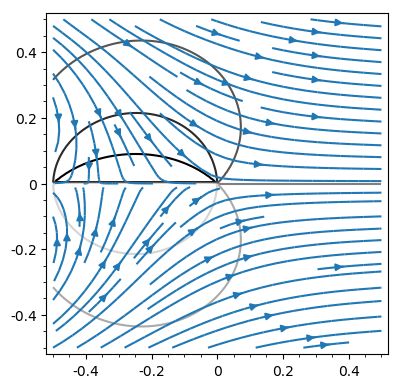
\includegraphics[width=0.3\textwidth]{B-05.png}}
                  \subfloat{
                   \label{f:conejo}
                    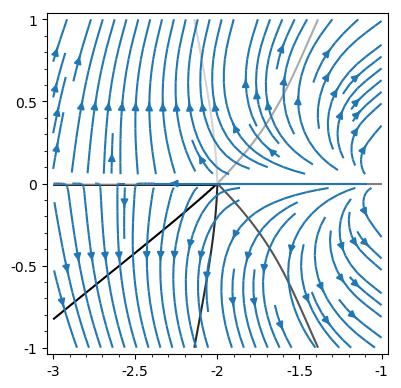
\includegraphics[width=0.301\textwidth]{B-2.png}}
            \end{figure}
        \end{itemize}
        
        \item Veure que per $z$ amb $|z|$ molt gran resulta $\Phi '(z) \approx \frac{1}{z+2}$ i que llavors lluny de $z = -2$ el flux associat a $\Phi '(z)$ és com una font sortint de $z = -2$.
        \begin{equation*}
            \begin{split}
                 \lim\limits_{|z|\to\infty} \Phi(z) & = \lim\limits_{|z|\to\infty} f(z) + \overline{f\left(\frac{1}{\overline{z}}\right)}\\
                        & = \lim\limits_{|z|\to\infty} \log(z+2) + \overline{\log\left(\frac{1}{\overline{z}}+2\right)}\\  
                        & = \lim\limits_{|z|\to\infty} \log(z+2) + \lim\limits_{|z|\to\infty} \overline{\log\left(\frac{z}{|z|^2}+2\right)}\\
                        & = \lim\limits_{|z|\to\infty} \log(z+2) + \log(2)
            \end{split}
        \end{equation*}
        Per tant, 
        \begin{equation*}
        \begin{split}
            \lim\limits_{|z|\to\infty} \Phi'(z) & \approx \lim\limits_{|z|\to\infty} \left( \log(z+2) + \log(2) \right)' \\
            & = \lim\limits_{|z|\to\infty} \frac{1}{z+2} 
            \end{split}
        \end{equation*}
        És a dir, veiem que com es deia a l'enunciat:
        $$\Phi'(z) \approx \frac{1}{z+2} \hspace{0.5 em} \text{quan} \hspace{0.5em } z \hspace{0.5em} \text{és molt gran.}$$
    
    \end{enumerate}
    \newpage
    \begin{enumerate}
        \item[\text{(d)}] Veure amb un gràfic com eviten el disc unitari les línies de flux (feu servir \textbf{contour\_plot} i \textbf{streamline\_plot}).
    \end{enumerate}
  \begin{figure}[h]
 \centering
  \subfloat{
   \label{f:gato}
    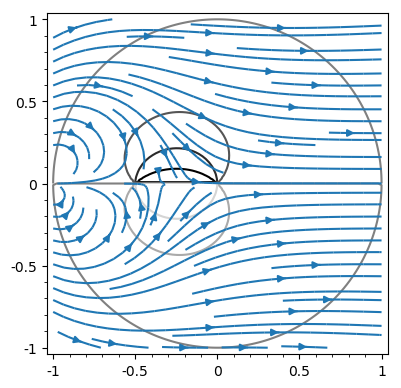
\includegraphics[width=0.3\textwidth]{2.png}}
  \subfloat{
   \label{f:tigre}
    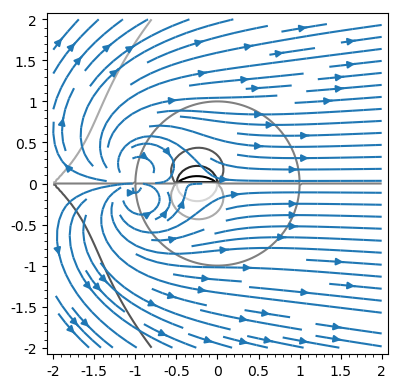
\includegraphics[width=0.3\textwidth]{1.png}}
  \subfloat{
   \label{f:conejo}
    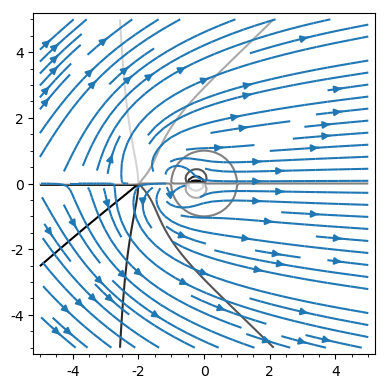
\includegraphics[width=0.291\textwidth]{3.png}}
 \caption{contour\_plot i sreamline\_plot de la funció}
 \label{13d}
\end{figure}
A les imatges adjuntades es poden observar les línies de flux de la funció $\Phi(z) = \log(z+2) + \log\left(\frac{1}{2}+z\right) - \log(z) + \log(2)$, amb diferents proximitats al disc unitari.\\
Com es pot observar, les línies de flux que surten de la $font$ situada al $-2$ i al $\frac{-1}{2}$ canvien de direcció, curvant-se en apropar-se al disc. Es pot veure que les línies sortints del $-2$ intenten seguir la vora del disc.\\
Per veure el codi utilitzat per generar les imatges, anar a l'apartat \textcolor{blue}{\ref{c13}}.\\
\clearpage
\section{Exercici 2.6.17 b)}
\begin{enumerate}
    \item[\text{(b)}] Discutir el moviment del fluid amb potencial complex igual a:
    \par
    $\Phi(z) = a\cdot z + \frac{\Gamma}{2\pi i} \cdot log(z) \hspace{0.5em} \text{on} \hspace{0.5em} a, \Gamma \in \mathbb{R}^+$
\end{enumerate}
\begin{table}[h]
    \centering
    \begin{tabular}{c | c | c | c }
        \diagbox{$a$}{$\Gamma$} & 1 & 50 & 100 \\\hline\hline
        \multirow{5}{*}{1} &  \multirow{5}{*}{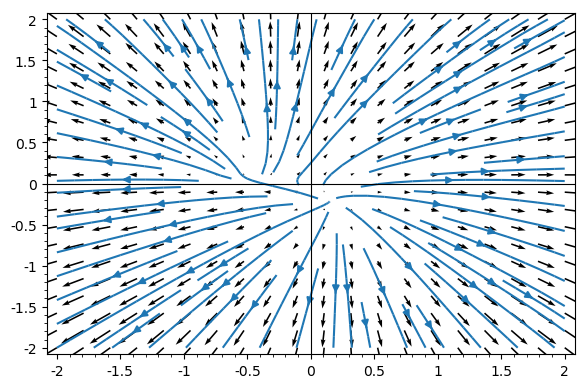
\includegraphics[width=0.25\textwidth]{a1_t1.png}} & \multirow{5}{*}{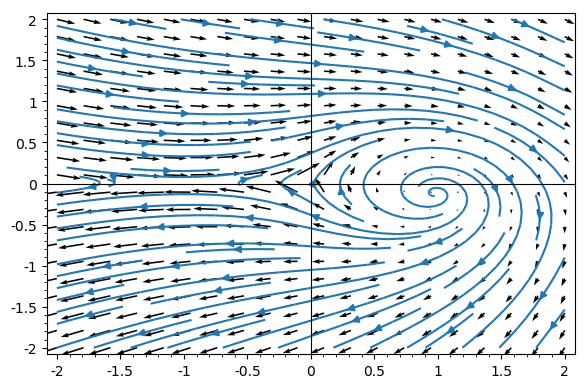
\includegraphics[width=0.25\textwidth]{a1_t50.png} }& \multirow{5}{*}{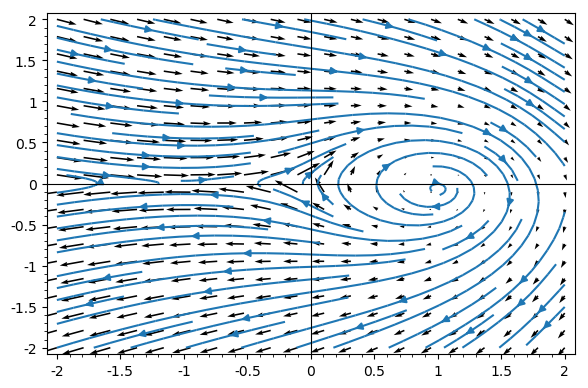
\includegraphics[width=0.25\textwidth]{a1_t100.png}} \\  
        &&&\\
        &&&\\
        &&&\\
        &&&\\\hline\hline
        \multirow{5}{*}{50} &  \multirow{5}{*}{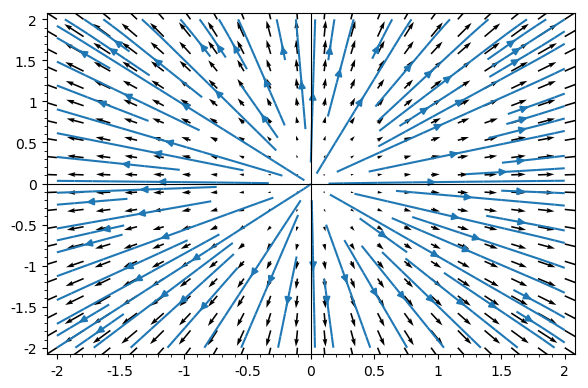
\includegraphics[width=0.25\textwidth]{a50_t1.png}} & \multirow{5}{*}{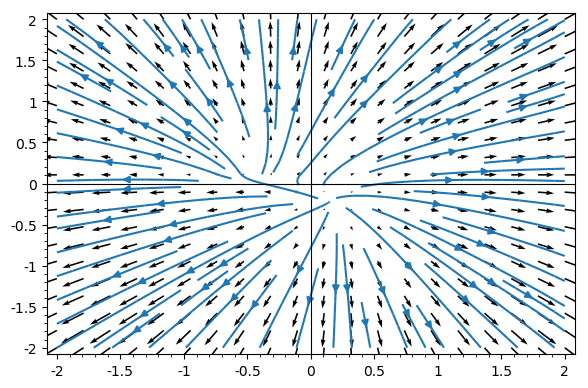
\includegraphics[width=0.25\textwidth]{a50_t50.png} }& \multirow{5}{*}{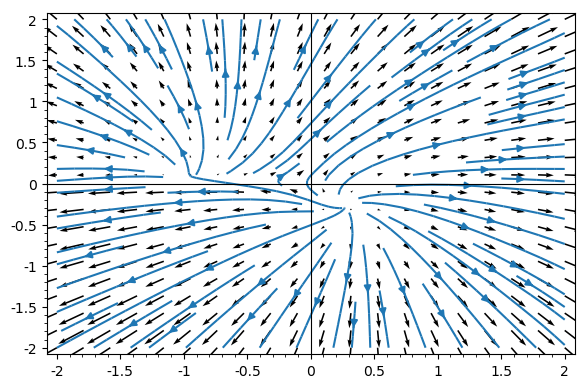
\includegraphics[width=0.25\textwidth]{a50_t100.png}} \\  
        &&&\\
        &&&\\
        &&&\\
        &&&\\\hline\hline
        \multirow{5}{*}{100} &  \multirow{5}{*}{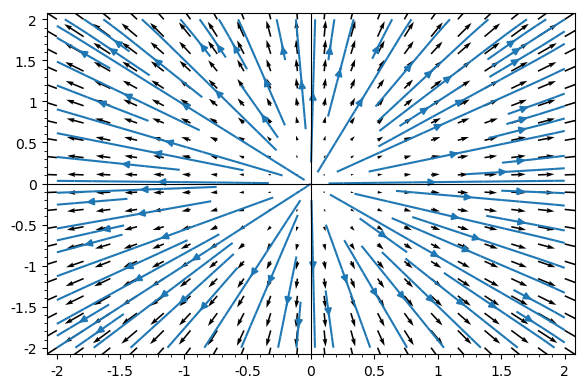
\includegraphics[width=0.25\textwidth]{a100_t1.png}} & \multirow{5}{*}{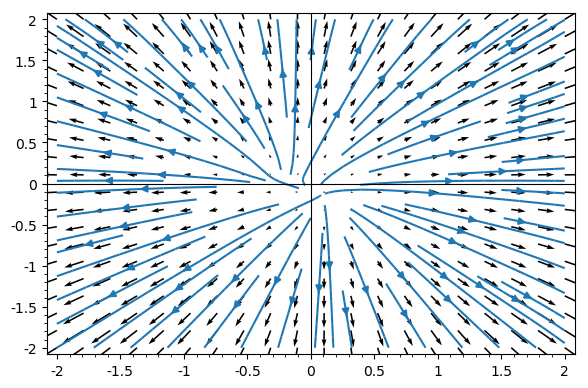
\includegraphics[width=0.25\textwidth]{a100_t50.png} }& \multirow{5}{*}{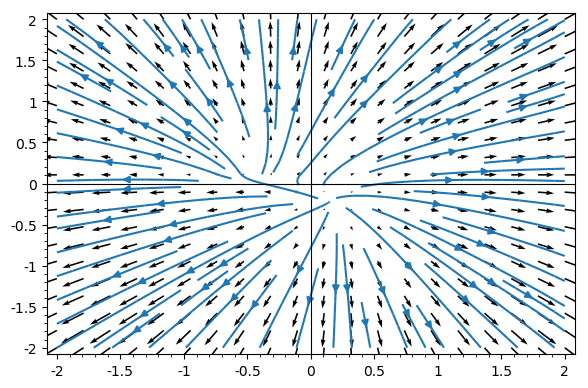
\includegraphics[width=0.25\textwidth]{a100_t100.png}} \\  
        &&&\\
        &&&\\
        &&&\\
        &&&\\
    \end{tabular}
    \caption{Gràfics de la funció per a diversos valors dels paràmetres $a$ i $\Gamma$}
    \label{17}
\end{table}
Per l'enunciat, $\Gamma > 0$, per tant sabem amb certesa que hi ha una $pica$.\\
Observem que quan el valor d'$a$ és major que $\Gamma$, els punts on es genera la $font$ i la $pica$ són molt propers (es mostra als gràfics només la $font$ ja que predomina sobre la $pica$).\\
En canvi, quan els valors d'$a$ i $\Gamma$ son iguals, els punts on s'originen la $font$ i la $pica$ es separen, fent que les línies de flux de la $font$ es curvin quan a causa de la $pica$, sent la curvatura més notoria a mida que aquesta és més propera a la $pica$.\\
Així doncs, veiem que quan augmenta el valor de $\Gamma$ (amb $\Gamma>a$) els punts on s'originen la $font$ i la $pica$ se separen, i els punts que les generen són molt diferenciats (per exemple en el cas $a=50, \Gamma=100$).\\
Però, quan el valor de $\Gamma$ és notablement més gran que el de $a$, ( exemples $a=1$ i $\Gamma=50,100$), la $pica$ i la $font$ són més distants. A més, tant la $font$ com la $pica$ adquereixen més "força" \hspace{0.1em} fent que mostrant sempre el mateix interval $(xmin, xmax)$, $(ymin,ymax)$ s'observi només la $pica$ i no la $font$ (ja que la $font$ no es genera dins d'aquest interval).\\
Per veure el codi utilitzat per generar les imatges de la taula llegir l'apartat \textcolor{blue}{\ref{c17}}.\\

\clearpage
\section{Exercici 2.6.18}

     Discutir el moviment del fluid amb potencial complex:
    \par
    $\Phi(z) = V_0 \cdot (z+\frac{R^2}{z}) + \frac{\Gamma}{2\pi i} \cdot log(z)
    \hspace{0.5em} \text{on} \hspace{0.5em} \Gamma, V_0, R \in \mathbb{R}^+$
\newline
Particularment estudieu els casos $\Gamma < 4\pi RV_0$, $\Gamma > 4\pi RV_0$ i $\Gamma = 4\pi RV_0$. Dibuixeu exemples de cadascun dels casos.
 \begin{figure}[h]
 \centering
  \subfloat[$\Gamma < 4\pi R V_0$]{
   \label{f:18peque}
    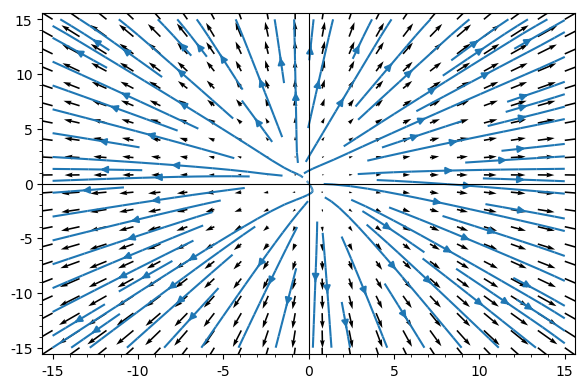
\includegraphics[width=0.3\textwidth]{18peque.png}}
  \subfloat[$\Gamma = 4\pi R V_0$]{
   \label{f:18mayor}
    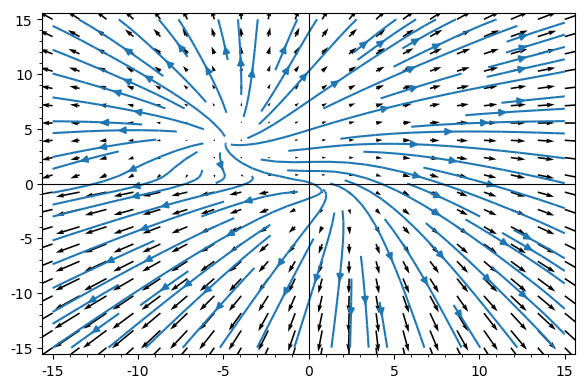
\includegraphics[width=0.3\textwidth]{18igual.png}}
  \subfloat[$\Gamma > 4\pi R V_0$]{
   \label{f:18mayor}
    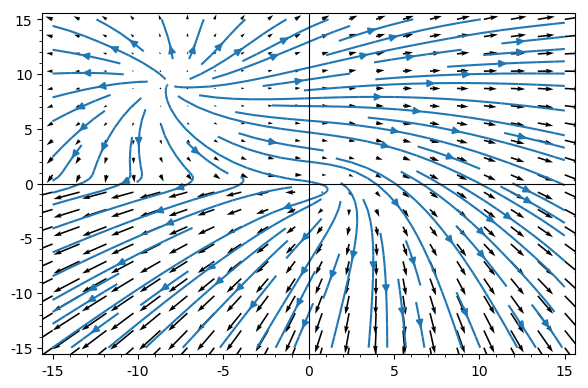
\includegraphics[width=0.3\textwidth]{18mayor.png}}
 \label{18}
 \caption{Representacions dels fluxos de corrent de la funció per a diversos valors de $\Gamma$}
\end{figure}
\\Per generar les imatges s'han utilitzat els valors $R=1$ i $V_0=1$.\\
Sabem que la primera part de l'expressió $\Phi(z)$, $V_0 \cdot (z+\frac{R^2}{z})$ genera una $font$, perquè es tracta d'una funció lineal. \\
En canvi, a la segona part de l'expressió $\frac{\Gamma}{2\pi i} \cdot log(z)$, veiem que la part real en aquest cas val $0$, i la part imaginària $Q = \frac{\Gamma}{2\pi i} = \frac{-\Gamma \cdot i}{2\pi}$. En ser $Q < 0$, es forma una $pica$.\\
Arrel d'això, com sabem que $Q$ va variant al llarg dels eixos, deduïm que en els tres casos a estudiar hi haurà tant una $font$ com una $pica$.
\begin{enumerate}[label=(\alph*)]
    \item S'ha utilitzat el valor $\Gamma = 4\pi-10$. 
    \\Els punts que generen la $pica$ i la $font$ són molt propers, de manera que podem observar les línies de flux de la $font$, que en apropar-se al $0$, prop de la $pica$, es curven.
    
     \item S'ha utilitzat el valor $\Gamma = 4\pi$. 
     \\Els punts que generen la $pica$ i la $font$ estan relativament allunyats l'un de l'altre. De manera que podem observar com les línies de flux de la $font$, a mesura que s'acosten més a la $pica$, augmenten la seva corbatura cap a la $pica$.
     
    \item S'ha utilitzat el valor $\Gamma = 4\pi+10$. 
    \\Com es pot veure a les diverses imatges, en augmentar el valor de $\Gamma$, els punts que generen la $pica$ i la $font$ estan significativament allunyats l'un de l'altre. Prop del $0$ s'hi troba la $pica$, mentre que la $font$ queda situada al segon quadrant. Això provoca que les línies sortints de la $pica$ canviïn de direcció en apropar-se al $0$.
\end{enumerate}
Per veure el codi utilitzat per generar les imatges, anar a l'apartat \textcolor{blue}{\ref{c18}}.\\

\newpage
\section{Codis}
\subsection{Exercici 2.4.13}
\hline
\begin{lstlisting}
def f(x,y):
    return imag(log(x+I*y+2)+log(1/2+(x+I*y))-log(x+I*y)+log(2))
def f2(x,y):
    return real(log(x+I*y+2)+log(1/2+(x+I*y))-log(x+I*y)+log(2))
    
var('x','y')

CP = contour_plot(f, (-1,0), (-0.5,0.5), fill=False)
SP = streamline_plot((f2,f), (-1,0), (-0.5,0.5))
show(CP+SP)

CP = contour_plot(f, (-0.5,0.5), (-0.5,0.5), fill=False)
SP = streamline_plot((f2,f), (-0.5,0.5), (-0.5,0.5))
show(CP+SP)

CP = contour_plot(f, (-3,-1), (-1,1), fill=False)
SP = streamline_plot((f2,f), (-3,-1), (-1,1)))
show(CP+SP)
\end{lstlisting}\label{c13}
\hline
\vspace{4em}
\subsection{Exercici 2.6.17 b)}
\hline
\begin{lstlisting}
def fr(x,y):
    return real(a*(x+I*y) + (T/(2*pi*I))*log(x+I*y))
def fi(x,y):
    return imag(a*(x+I*y) + (T/(2*pi*I))*log(x+I*y))
    
var('x', 'y')
A = 2 

for a in (1,50, 100):
    for T in (1,50, 100):
        CP = plot_vector_field((fr,fi), (-A,A), (-A,A))
        SP = streamline_plot((fr,fi), (-A,A), (-A,A)
        show(CP+SP)
\end{lstlisting}\label{c17}
\hline
\newpage
\subsection{Exercici 2.6.18}
\hline
\begin{lstlisting}
def g(x,y):
    return real(V0*((x+I*y)+(R^2)/(x+I*y))+(T/(2*pi*I))*log(x+I*y))
def g2(x,y):
    return imag(V0*((x+I*y)+(R^2)/(x+I*y))+(T/(2*pi*I))*log(x+I*y))
    
var('x','y')
V0=1
R=1

for T in (4*pi*R*V0-10, 4*pi*R*V0, 4*pi*R*V0+10):
    CP = plot_vector_field((g,g2), (-15,15), (-15,15))
    SP = streamline_plot((g,g2), (-15,15), (-15,15))
    show(CP*SP)
\end{lstlisting}\label{c18}
\hline

\end{document}
